\documentclass[border=10pt]{standalone}

\usepackage{tikz}
\usepackage{tikzsymbols}
\usetikzlibrary{calc,patterns,shapes.geometric}

\def\centerarc[#1](#2)(#3:#4:#5){\draw[#1] ($(#2)+({#5*cos(#3)},{#5*sin(#3)})$) arc (#3:#4:#5);}

\begin{document}
	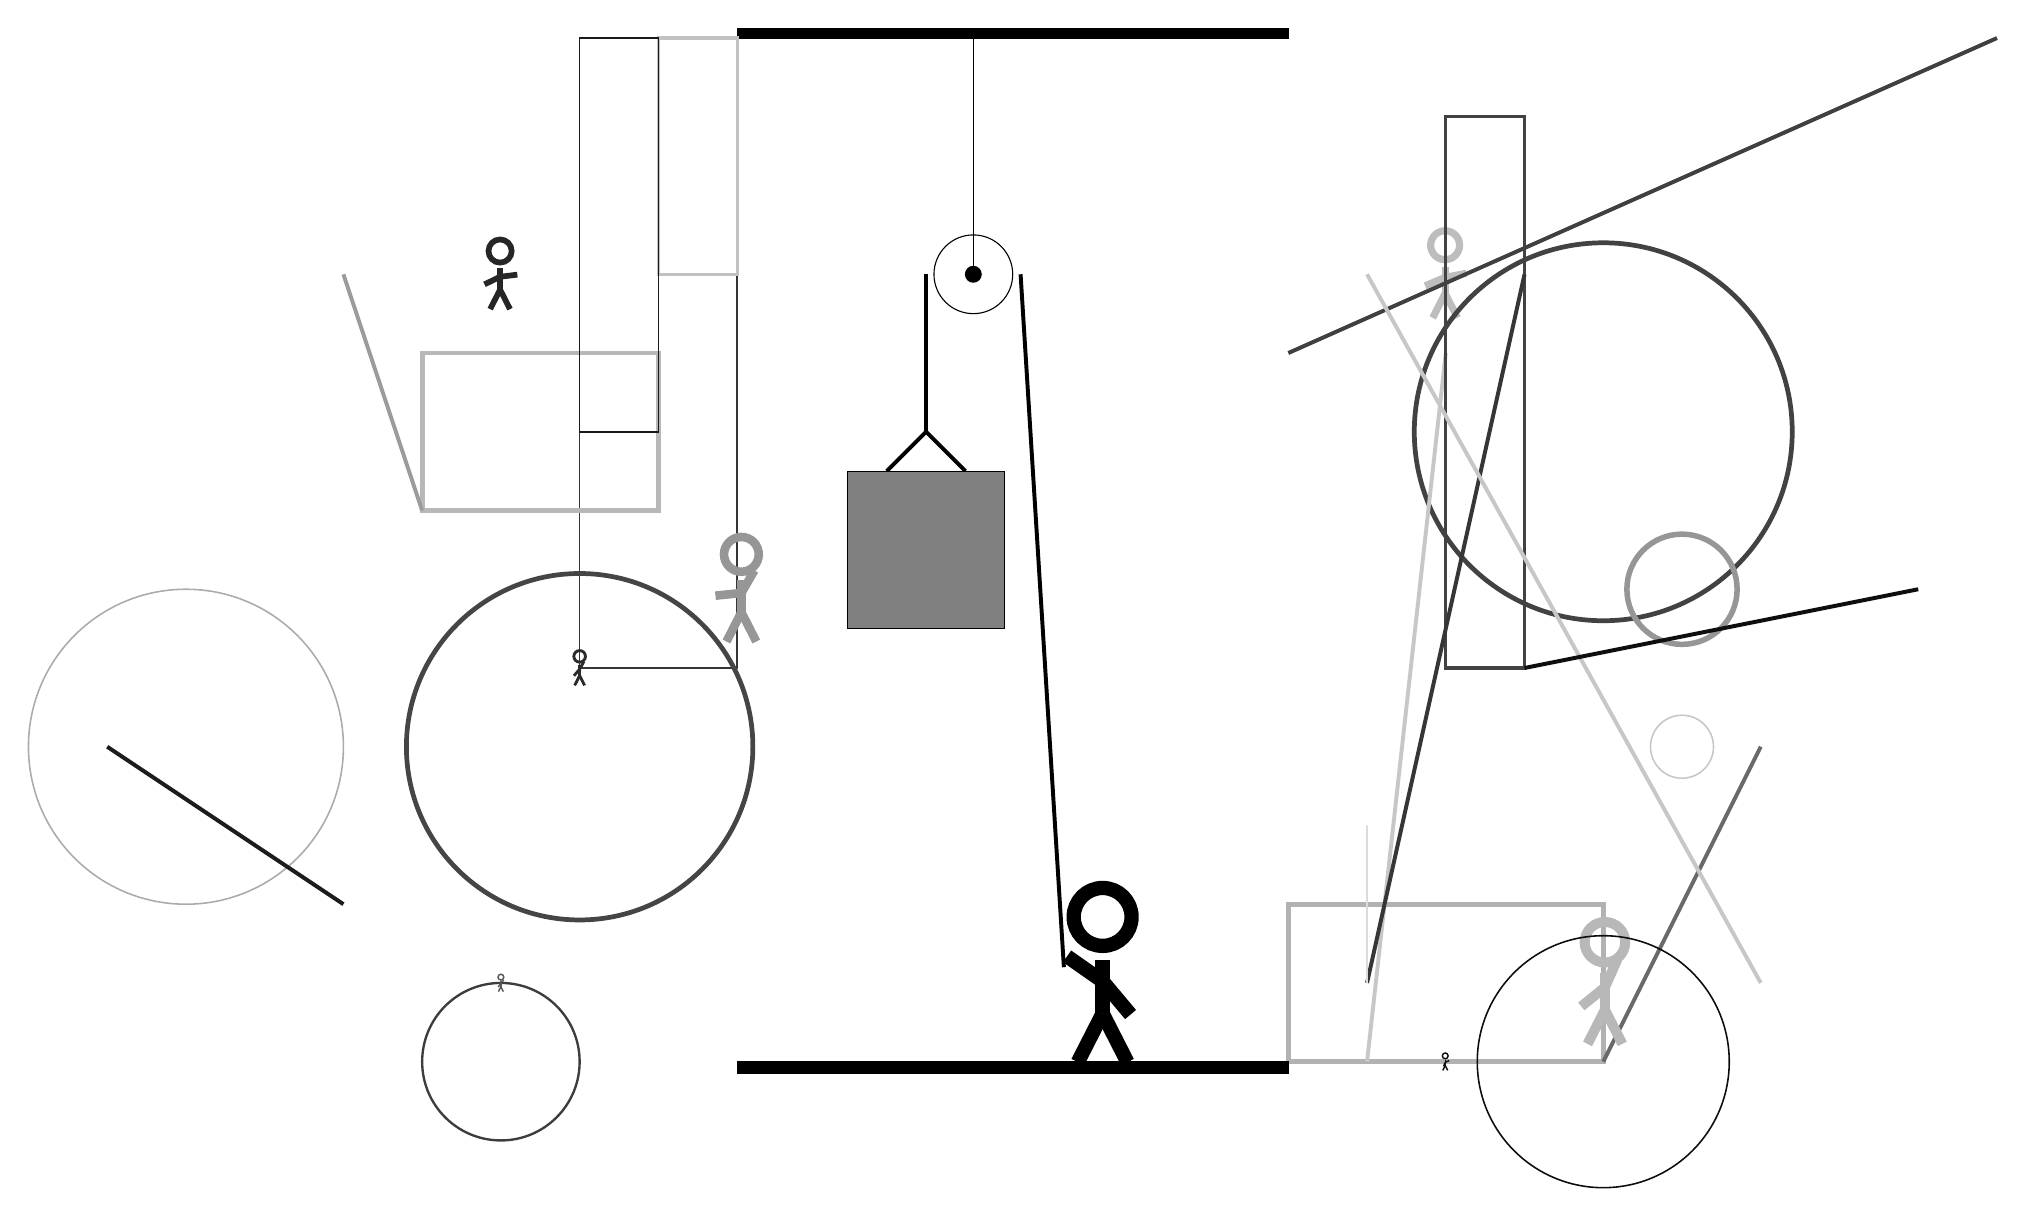
\begin{tikzpicture}
		%%%%% START %%%%%
		
		\draw[fill=black] (-2, 10) rectangle (5, 10.125);
		
		\draw (1, 7) circle (0.5);
		\draw[fill=black] (1, 7) circle (0.1);
		\draw (1, 10) -- (1, 7);
		
		\draw[line width=0.5mm] (-0.1, 4.5) -- (0.4, 5.0) -- (0.9, 4.5);
		\draw[fill=black!50] (-0.6, 4.5) rectangle (1.4, 2.5);
		
		\draw[line width=0.5mm] (0.4, 7) -- (0.4, 5.0);
		\centerarc[line width=0.5mm](1, 7)(0:180:0.6);
		\draw[line width=0.5mm](1.6, 7) -- (2.15, -1.8);
		
		\node at (2.6, -1.9) {\Strichmaxerl[10][-35][-50]};
		
		\node[line width=0.4mm, color=black!85] at (-5, 7) {\Strichmaxerl[4][26][7]};
		
		\draw[line width=0.6mm, color=black!30] (5, -3) rectangle (9, -1);
		\draw[line width=0.2mm, color=black!79] (-4, 10) rectangle (-2, 2);
		\node[line width=0.5mm, color=black!83] at (-4, 2) {\Strichmaxerl[2][49][61]};
		
		\draw [line width=0.6mm, color=black!73](-4, 1) circle (2.2);
		\node[line width=0.4mm, color=black!26] at (7, 7) {\Strichmaxerl[5][23][11]};
		
		\draw [line width=0.3mm, color=black!76](-5, -3) circle (1.0);
		
		\node[line width=0.7mm, color=black!66] at (-5, -2) {\Strichmaxerl[1][50][52]};
		\draw [line width=0.6mm, color=black!74](9, 5) circle (2.4);
		
		\draw[line width=0.4mm, color=black!24] (-3, 7) rectangle (-2, 10);
		\draw[line width=0.5mm, color=black!59](9, -3) -- (11, 1);
		\draw[line width=0.5mm, color=black!75](5, 6) -- (14, 10);
		\draw [line width=0.2mm, color=black!70](-9, 3) circle (0.0);
		\node[line width=0.7mm, color=black!28] at (9, -2) {\Strichmaxerl[7][39][66]};
		\draw [line width=0.2mm, color=black!95](9, -3) circle (1.6);
		\node[line width=0.2mm, color=black!94] at (7, -3) {\Strichmaxerl[1][67][24]};
		
		\draw [line width=0.2mm, color=black!22](10, 1) circle (0.4);
		
		\draw[line width=0.5mm, color=black!22](7, 6) -- (6, -3);
		\draw[line width=0.6mm, color=black!28] (-3, 4) rectangle (-6, 6);
		\draw[line width=0.5mm, color=black!39](-6, 4) -- (-7, 7);
		\draw [line width=0.7mm, color=black!41](10, 3) circle (0.7);
		
		\draw[line width=0.4mm, color=black!74] (7, 9) rectangle (8, 2);
		\draw[line width=0.5mm, color=black!79](8, 7) -- (6, -2);
		\draw[line width=0.5mm, color=black!22](6, 7) -- (11, -2);
		\draw[line width=0.3mm, color=black!14] (6, -2) rectangle (6, 0);
		\draw [line width=0.2mm, color=black!33](-9, 1) circle (2.0);
		
		\node[line width=0.2mm, color=black!41] at (-2, 3) {\Strichmaxerl[6][6][60]};
		\draw[line width=0.2mm, color=black!90] (-3, 10) rectangle (-4, 5);
		\draw[line width=0.5mm, color=black!89](-7, -1) -- (-10, 1);
		\draw[line width=0.5mm, color=black!94](8, 2) -- (13, 3);
		
		\draw[fill=black] (-2, -3) rectangle (5, -3.15);
		
		%%%%% END %%%%%
	\end{tikzpicture}
\end{document}